\documentclass[10pt]{article}

\usepackage[T1]{fontenc}
\usepackage[utf8]{inputenc}
\usepackage[margin=1in]{geometry}
\usepackage{graphicx}
\graphicspath{{sections/}}
\usepackage{float}
\usepackage[hidelinks]{hyperref}

\title{Ephemeral Sandbox: A LayerStack Workspace OS for Parallel Coding Agents\\
  \large\textit{Provisional working title}}
\author{\texttt{[AUTHOR INFORMATION NEEDED]}\\
  \texttt{[AFFILIATION INFORMATION NEEDED]}}
\date{Draft manuscript scaffold}

\begin{document}

\maketitle

\begin{abstract}
\noindent\textbf{Provisional design-first draft---not submission text.}
Agent systems can fan out intelligence, but conventional operating-system
workspaces provide no agent-level protocol for fanning concurrent writes back
into one durable project. Coding-agent teams and swarms inspect changing code,
perform multi-file edits, run tests, and start services; sharing one mutable
workspace permits live-state interference, while copying workspaces alone
defers integration. We present Ephemeral Sandbox, a workspace OS organized
around LayerStack: one durable project history, many private executable
sessions, and controlled publication. A sessionless
\texttt{exec\_command} tool call receives an implicit isolated session over a
leased LayerStack snapshot. When its command ledger drains, the runtime
captures the private overlay, reconciles the complete delta against the current
head, and either publishes one new layer or returns a structured rejection.
Eligible text divergence can use a bounded three-way merge; structural,
binary, oversized, or conflicting changes reject. Explicit sessions let
multiple command and file tool calls share private state before publication or
discard. Source and correctness tests establish these mechanisms, but not
formal security, semantic merge correctness, process-state rollback, resource
coordination, or improved multi-agent throughput. Whether Ephemeral Sandbox
raises the workload-dependent useful-work concurrency ceiling remains an
empirical question.
\end{abstract}

\section{Introduction}
\label{sec:introduction}
\emph{Draft.}

\section{Goals, Non-goals, and Threat-model Boundary}
\label{sec:goals-nongoals}
\emph{Draft.}

\section{System Model and Invariants}
\label{sec:system-model}
\emph{Draft.}

\section{Workspace Execution}
\label{sec:workspace-execution}

Workspace creation begins by acquiring a snapshot lease, not by reading an
unprotected copy of the current head.  The lease records the selected manifest
and its resolved ordered layer paths; the workspace handle carries that
snapshot together with session-unique runtime directories.  Only after this
view has been fixed does the runtime open the executable workspace.  A later
publication may advance the active manifest, but it does not change the
manifest or layer ordering observed through the live session's lease.  This is
the concrete mechanism behind the stable-view invariant in
Section~\ref{sec:system-model}, without importing serializable snapshot
isolation.

On the supported Linux path, the runtime projects the leased LayerStack with
OverlayFS.  The manifest's layers become read-only lower directories in
newest-first precedence order, while the session receives a unique upper
directory and work directory.  The resulting mount therefore reads through
shared history but records regular writes, copied-up files, and deletion or
opacity metadata only in the private upper tree.  Lower layers are shared
runtime state; the upper/work pair is session-private state.  This mechanism
is Linux- and OverlayFS-centered at the audited baseline: the non-Linux mount
path reports the operation as unsupported, and the paper makes no universal
cross-platform execution claim.

Each workspace also has a long-lived namespace-holder process.  The holder
creates and keeps open the session's user, mount, and PID namespaces and, when
selected, its network namespace.  The daemon retains file descriptors for
these namespaces rather than moving its own control process into them.  For
each command, a short-lived runner joins the recorded user, mount, PID, and
optional network namespaces in the runtime's required order and launches the
command against the already mounted workspace.  This holder/runner split lets
successive commands enter the same filesystem and process-namespace context
while the daemon remains outside the command namespaces.  It is an
implementation isolation boundary, not a proof that hostile code cannot
escape or interfere through every host resource.

A sessionless \texttt{exec\_command} uses the \emph{implicit session} path.
The operation service creates a workspace with the shared-network profile and
a publish-then-destroy finalization policy, admits the requested command, and
tracks it in the session's command ledger.  Publication is eligible only after
the active-command set becomes empty and the ledger reaches its drained
terminal state; it is therefore tied to command completion, not merely to
returning an initial command handle or response.  The finalizer then attempts
the capture, publication, and destruction phases described below.  This
automatic lifecycle is specific to sessionless command execution.

An \emph{explicit session} instead keeps one leased view, namespace holder,
mount, and private upper/work pair across multiple calls.  Commands admitted
with its session identifier and file operations directed to that session
observe the same live overlay, so later operations can consume earlier private
writes before anything reaches the active head.  The explicit session uses a
no-op automatic finalization policy: its caller deliberately requests
publication or destruction.  Publication admission fails while commands are
still active, preventing capture from racing an admitted command through the
normal service path.

File and network qualifiers matter to this account.  A session-scoped read,
write, or edit operates on the live mounted workspace and therefore on the
private overlay.  A sessionless read instead projects the latest published
LayerStack, while a sessionless write or edit directly amends the current head
with a one-layer operation under the LayerStack writer lock; neither
sessionless file path creates an implicit workspace session.  Likewise,
shared networking joins the host network namespace while retaining separate
user, mount, and PID namespaces, whereas the isolated profile creates a
separate network namespace and its configured connectivity.  Shared
networking is consequently not an egress-containment guarantee, and selectable
network isolation is not evidence of universal denial policy.

Workspace creation has several externally fallible steps---lease acquisition,
directory allocation, holder startup, namespace access, overlay mounting, and
optional network setup.  The service attempts to roll back resources created
before a failed admission, while a successfully admitted session retains its
lease and private tree until its lifecycle reaches cleanup.  Neither path
captures command registers, memory, sockets, or an arbitrary process tree for
later rollback.  Publication begins only from the filesystem delta left in the
complete private upper directory; the next section follows that delta from
capture to the active head.

\section{Capture and Publication}
\label{sec:capture-publication}

Capture walks the complete private upper tree and converts OverlayFS
representations into typed layer changes.  Regular files become write records
that retain a source path and size so publication can stream their bytes;
symbolic links, directory entries, and empty directories remain typed
entries.  Kernel whiteouts---character devices with device number zero or the
supported whiteout extended attribute---become deletions, while the supported
opaque-directory extended attributes become opaque-directory changes.  An
ordinary name beginning with \texttt{.wh.} is not reinterpreted as a
capture-time marker; it remains a path and is rejected later because that name
space is reserved by the layer format.  Invalid layer paths and unsupported
special files are reported as protected drops rather than silently converted.
Explicit-session publication rejects any such drop.  The lower-level planner
has a narrower exception for an unsupported-special-file drop, so the source snapshot
does not yet justify one uniform protected-drop policy across every
publication entry point.

\begin{figure}[t]
\centering
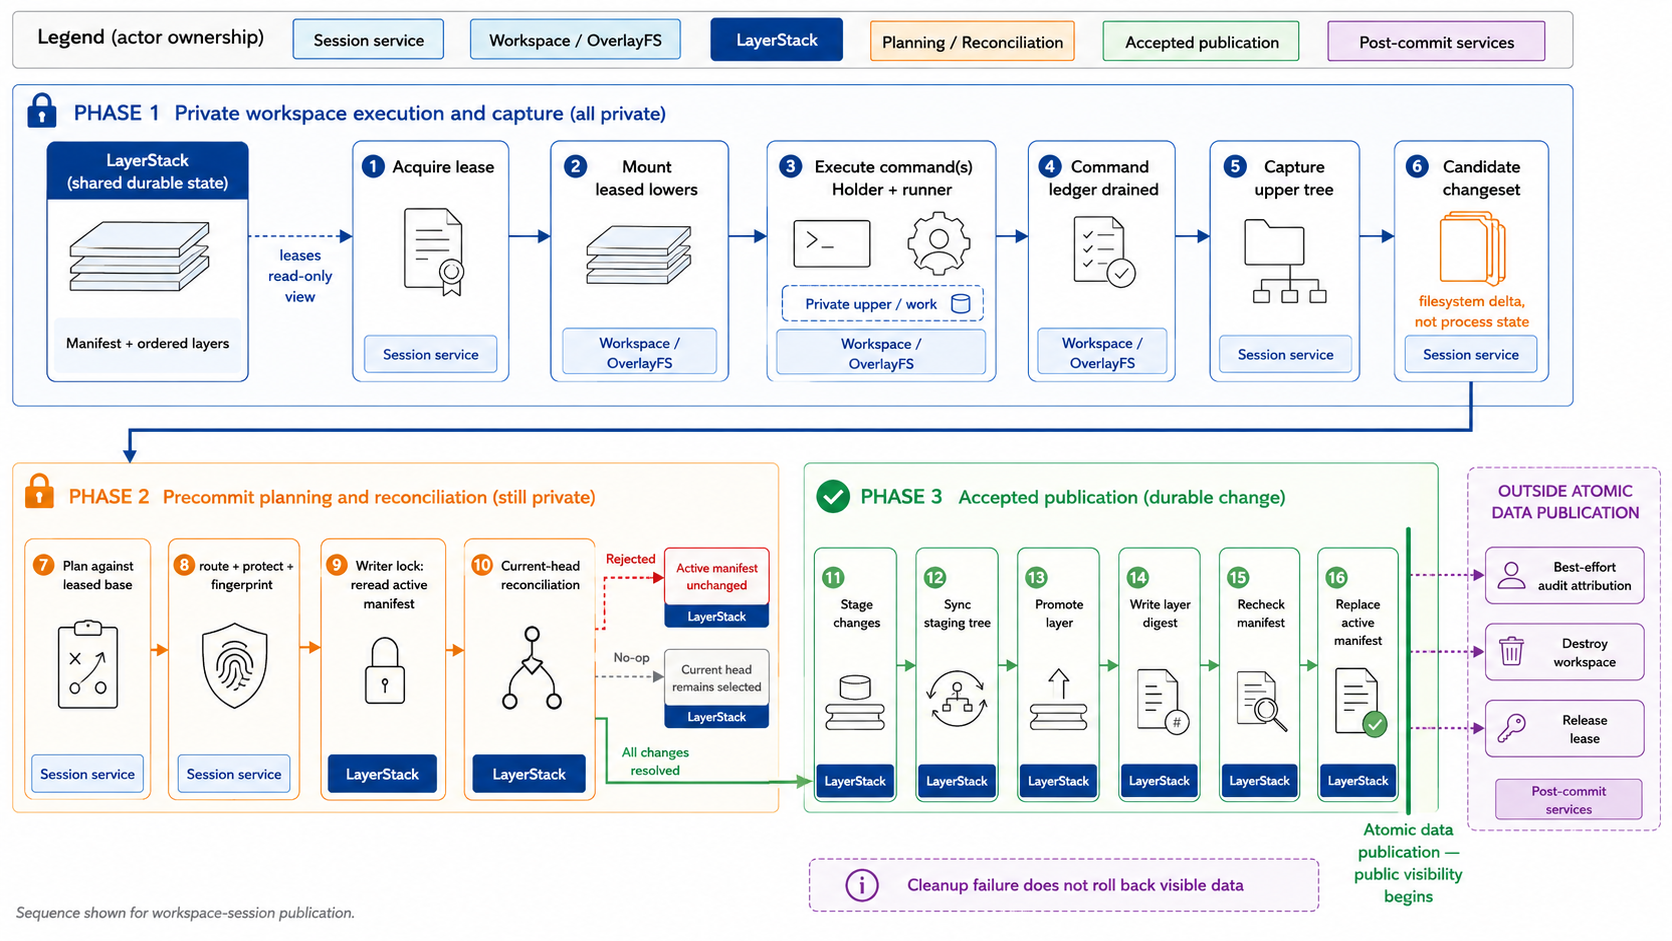
\includegraphics[width=\linewidth]{../figures/concept/fig_publication_sequence.png}
\caption{Workspace-session publication sequence.  Execution, ledger drain,
capture, and current-head reconciliation remain private or precommit.  Public
data visibility begins at active-manifest replacement; best-effort attribution,
workspace destruction, and lease release follow outside the atomic data
publication boundary.  The sequence does not describe sessionless direct file
amendment.}
\label{fig:publication-sequence}
\end{figure}

Planning evaluates the candidate against the leased base before taking the
commit lock.  It verifies that the supplied manifest version, root hash, and
layer count describe the same base manifest.  Each path is then routed as
source or ignored according to the base view's ignore policy, and reserved
runtime paths---including the manifest, layer and staging directories,
\texttt{.layer-metadata}, and \texttt{.wh.*} components---cause rejection.
Source-routed paths receive content fingerprints from the leased base.
Planning an opaque directory additionally enumerates the lower descendants it
would hide: a protected descendant, a mixture of source and ignored routes, or
an expansion beyond the fixed bound rejects the candidate.  These checks turn
a captured delta into an explicit plan; they do not yet make it durable.

The service then acquires the LayerStack writer lock, rereads the active
manifest, and resolves source validations against that current head.  A source
path whose current fingerprint still matches its base fingerprint is accepted
as planned; an idempotent concurrent creation of the same directory is also
compatible.  Changes that replace or obscure a directory trigger descendant
checks so a concurrent change below that path cannot be erased unnoticed.
Other structural differences reject the publication.  Ignored-route changes
are carried as wholesale writes and do not receive the source fingerprint and
merge treatment.  The policy is thus conflict-aware for source state while
making its separate ignored-state route explicit, rather than claiming a
general database isolation level.  Figure~\ref{fig:reconciliation-decision}
expands these route and resolution decisions.

\begin{figure}[t]
\centering
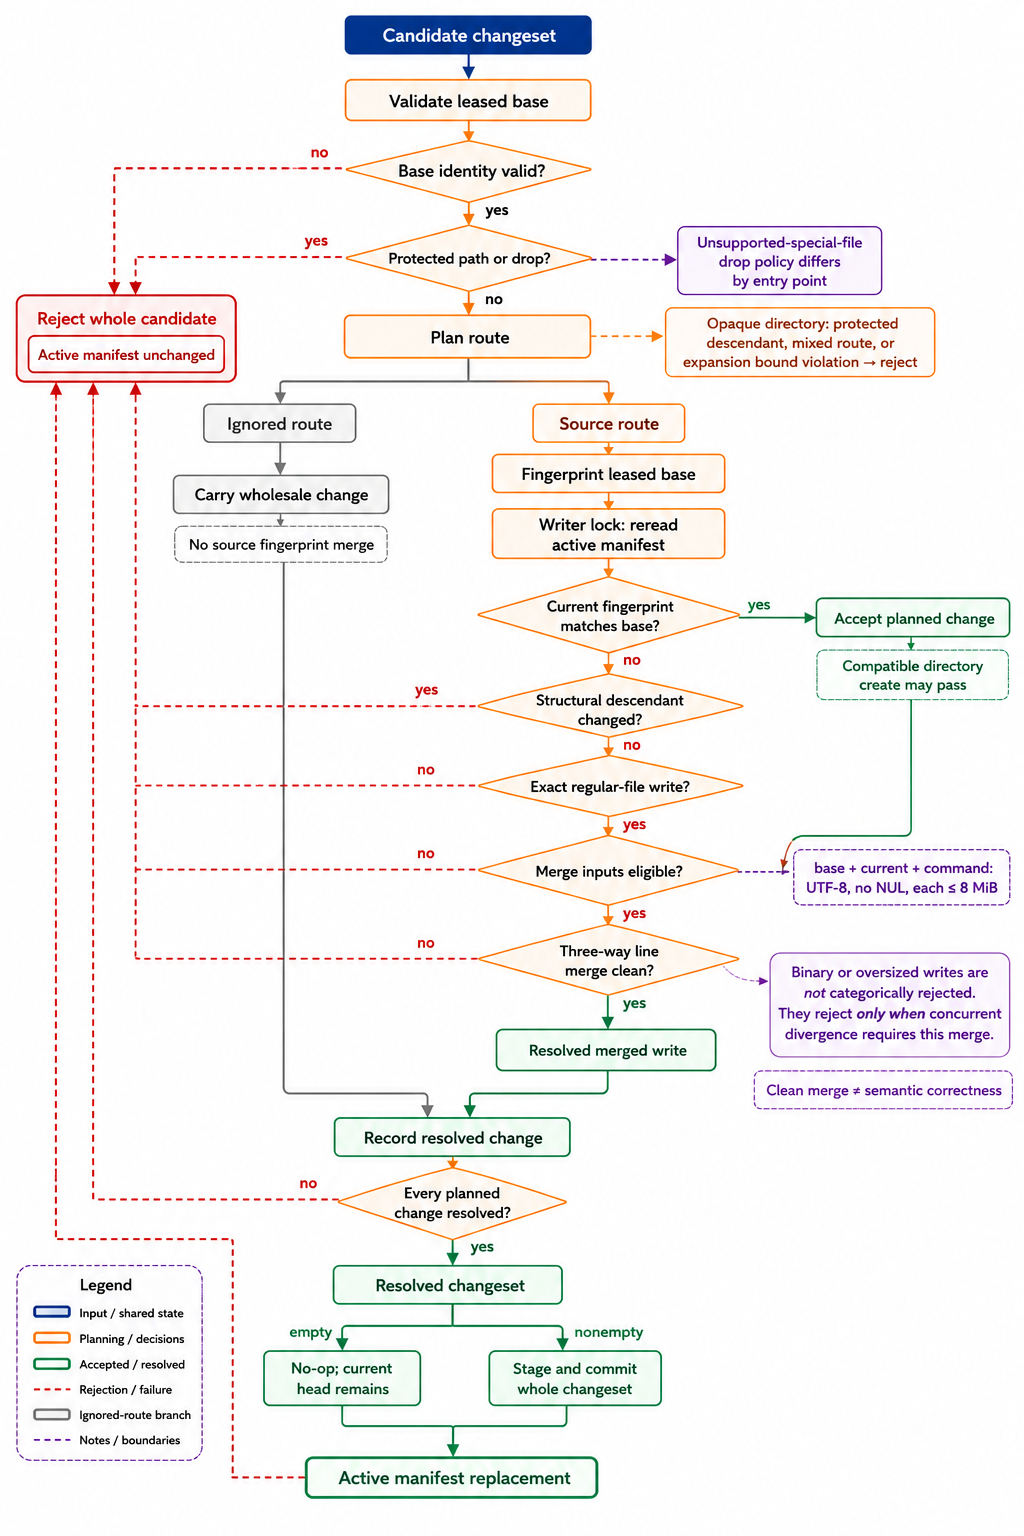
\includegraphics[height=0.82\textheight]{../figures/concept/fig_reconciliation_decision.png}
\caption{Current-head reconciliation decision flow.  Source-routed changes
receive base/current fingerprint and structural checks, and only eligible
exact-file textual divergence reaches three-way line merge.  Every planned
change must resolve before a nonempty changeset is committed; otherwise the
whole candidate is rejected and the active manifest remains unchanged.  A
no-op retains the current head and is not a new data publication.}
\label{fig:reconciliation-decision}
\end{figure}

When a source fingerprint has diverged, the only merge-eligible candidate is a
regular-file write at that exact path.  The resolver reads the leased-base,
current-head, and command versions and applies a three-way line merge only
when each is valid UTF-8 text without NUL bytes and no larger than 8 MiB.
Disjoint edits, or overlapping edits with byte-identical replacement lines,
can yield a clean merged file; differing overlapping edits reject it.  A
non-file transition, binary content, invalid UTF-8, an oversized input, or a
text conflict is ineligible when reconciliation requires this merge and
therefore becomes a source conflict.  By contrast, a binary or oversized
write whose source fingerprint has not diverged can still publish without a
merge.  A clean line merge establishes only structural compatibility: it is
not a semantic-correctness guarantee, and the byte threshold alone is not a
claim that worst-case diff CPU or memory is adequately bounded.

Resolution constructs one final changeset or returns one rejection; no
resolved subset escapes to the layer writer.  Protected paths, invalid base
identity, opaque-directory violations, structural source changes, and
ineligible or conflicting required merges therefore leave the active manifest
unchanged.  An empty resolved changeset is a no-op at the current head.  For an
explicit session, lifecycle handling after a capture or publication failure is
separate from this resolution decision and belongs to
Section~\ref{sec:lifecycle-recovery}.  The data outcomes provide all-or-none
handling without calling the session a full transaction.

For a nonempty resolved changeset, the layer writer first computes its digest
and recognizes an identical current head as a no-op.  Otherwise it writes the
changes beneath a newly allocated staging directory, synchronizes regular
files and the staging tree, renames that tree into the durable layer store, and
synchronizes the layer directory's parent.  It then writes the layer digest,
rereads the active manifest to detect an intervening replacement, and builds a
new manifest whose first entry is the promoted layer.  The manifest writer
creates and synchronizes a temporary file, renames it over the active manifest,
and synchronizes the containing directory.  Only this final replacement makes
the resolved layer part of the active head.  Failures before it can leave
recoverable staging or unreferenced artifacts, but they do not select the new
layer in the active manifest.

The successful manifest replacement is the end of \emph{atomic data
publication}, not the end of the session lifecycle.  After the layer commits,
the operation service maps structural line origins to an owner and appends
per-path audit events.  That attribution is deliberately best effort: an audit
append failure does not fail or roll back the visible data.  The service then
begins the separate workspace-destruction and lease-release phase.  Accounting,
observability events, autosquash notification, session cleanup, and later
garbage collection likewise remain outside the all-or-none data boundary;
Section~\ref{sec:lifecycle-recovery} defines their failure outcomes.

This path explains how one private filesystem delta can become one durable
public head at the audited Linux source snapshot. It does not establish
semantic merge correctness, a cross-platform crash proof, or an unlimited
transaction size. Staging remnants, retained sessions, lease release, cleanup
failure, compaction, and reclamation are lifecycle and recovery concerns,
which Section~\ref{sec:lifecycle-recovery} treats separately.

\clearpage

\section{Lifecycle and Recovery}
\label{sec:lifecycle-recovery}
\emph{Draft.}

\section{Implementation and Operational Interface}
\label{sec:implementation-interface}

\subsection{Source-Derived Operational Cost Model}
\label{sec:cost-model}

Ephemeral Sandbox does not have one context-free time or space complexity.
Each session passes through stages with different scaling variables.  Let
$L$ be manifest depth, $S$ the number of live sessions, $U$ the number of
private-upper entries, $C$ the number of captured changes, $F$ the number of
validated source paths, $B_p$ the logical regular-file bytes published, $Q$
the number of concurrent publishers, and $R=\sum_{i=1}^{S}L_i$ the layer
references retained across live leases.  Table~\ref{tab:cost-model} records
source-derived drivers; it is not a performance result.

\begin{table}[t]
\centering
\small
\begin{tabular}{p{0.19\linewidth}p{0.36\linewidth}p{0.34\linewidth}}
\hline
Stage & Time driver & Live or peak space driver \\
\hline
Session creation &
$O(L)$ manifest cloning, path resolution, lower validation, and mount
configuration in userspace &
$O(L)$ metadata per lease/session and $O(R)$ across live leases; fresh
upper/work directories do not eagerly copy the project \\
Capture &
$O(U)$ metadata/path work plus per-directory sorting &
$O(U)$ change metadata; regular-file payload remains referenced on disk \\
Plan/resolve &
Changed-path routing and repeated layered fingerprint probes; eligible merge
depends on line count and edit distance &
Fingerprints and validations scale with $C+F$; merge retains file, line,
edit, output, origin, and trace state \\
Commit &
$O(C\log C)$ path aggregation, at least $O(B_p)$ byte hashing/copy/sync, and
$O(L)$ manifest work under one writer &
The private upper can coexist with staging/final publication data; each
unsquashed publish adds a manifest layer \\
Squash/GC &
Manifest/lease planning, layered directory traversal, then a brief serialized
commit &
Replacement metadata coexists with old layers; leases retain otherwise
obsolete history until safe release \\
\hline
\end{tabular}
\caption{Operational cost model derived from the v1 source.  Logical bytes are
not physical allocated bytes; the latter requires filesystem measurements.}
\label{tab:cost-model}
\end{table}

The durable head transition is serialized by design.  In v1, the exclusive
writer section includes active-head resolution, eligible text reconciliation,
payload hashing and copying, synchronization, promotion, and manifest
replacement.  Private execution can therefore remain parallel while
publication wait grows with $Q$, $B_p$, $F$, or merge work.  This is a
mechanism-level saturation hypothesis, not evidence that publication is the
limiting stage for any workload.

Text reconciliation is bounded to 8\,MiB per input, but that byte gate is not
an independent memory bound for the line diff.  For total line count $n$,
reached edit distance $D$, and $K=\min(n,200{,}000)$, the current implementation
retains an $O(KD)$ frontier trace and can approach an $O(K^2)$ trace envelope.
The evaluation must stress line count and edit shape in addition to file bytes.

\subsection{Operational Interface}

\emph{Draft pending PW3.  This subsection will describe the role-separated
management, runtime, and read-only observability clients and the final tagged
catalog-derived contract.}

\section{Evaluation}
\label{sec:evaluation}

\subsection{RQ3: Latency, Storage, and Resource Scaling}

RQ3 tests the source-derived cost model rather than assuming that worker count
alone explains scaling.  The protocol independently varies worker/publisher
count, manifest depth, live-session count and lease age, private-upper entry
count and fan-out, changed and validated paths, published logical bytes,
conflict class, and eligible-merge bytes, lines, similarity, and edit distance.
Storage cases include small edits to large files, many small files, and
incompressible controls.  All factors, warmups, repeats, and stopping rules
must be fixed before the final source freeze.

For each stage, we report latency distributions, CPU, RSS/PSS, I/O, failures,
and exact phase boundaries.  Publication additionally reports writer-lock wait
and hold time and decomposes planning, resolution/merge, hashing, copy,
synchronization, and manifest transition.  Storage reports logical, allocated,
shared, and exclusive bytes for upper, work, staging, published layers, and
lease-retained history.  Squash reports plan, build, commit, and garbage
collection separately.  No cost-model term becomes a paper result until it is
reproduced from frozen raw artifacts and analysis code.

\emph{The remaining RQ1--RQ5 methodology and all numerical results are pending
protocol and evidence lock.}

\section{Limitations and Related Work}
\label{sec:limitations-related-work}

\subsection{Limits of the Present System and Evidence}

The system isolates workspace effects; it does not solve task decomposition,
model quality, semantic compatibility, verification, service ownership, or
general agent coordination. Publication is intentionally serialized, and its
critical path includes active-head reconciliation, eligible text handling,
payload hashing and copying, synchronization, and manifest replacement.
Long-lived leases can retain historical layers, while path validation and merge
work depend on the shape of the changed tree. The implementation's bounded
text merge is not an independently bounded line- or edit-trace memory
algorithm. These are design limitations, not measurements of a general
concurrency ceiling.

The copy-on-write workspace abstraction also does not imply negligible physical
storage. Copy-up, sparse allocation, compression, extent sharing, page cache,
and metadata are backend dependent; a small edit can materialize a large
logical upper file. The frozen evaluation consequently reports only its
observed resource counters and workspace deltas. It does not establish a
capacity reservation, a storage-saving claim, a security boundary, or behavior
on operating systems and filesystems not covered by the campaign.

LayerStack evolution remains future work. In particular, the paper does not
claim reflink support, process-state rollback, transactional publication
attribution, daemon-restart recovery, or semantic merge correctness. A future
evaluation needs heterogeneous projects, controlled competing systems,
publication and recovery faults, larger concurrency and history sweeps, and
end-to-end collaborative coding outcomes.

\subsection{Isolation, Reversibility, and Agent Runtime Substrates}

Several systems already provide isolated environments for software agents.
SWE-MiniSandbox develops container-free isolated workspaces for software
engineering-agent training, while AgentBay exposes hybrid human and agent
control over sandbox sessions \cite{swe_minisandbox_2026,agentbay_2025}. They
motivate isolated execution but do not make this paper's runtime-publication
claim. DeltaBox focuses on change-based sandbox checkpoint and rollback,
including process state, and Shepherd records reversible agentic execution
traces for fork and replay \cite{deltabox_2026,shepherd_2026}. Ephemeral
Sandbox does not implement complete process-state checkpointing, rollback, or
replay; its claim is restricted to private filesystem workspace state followed
by controlled durable publication.

\subsection{Concurrent Coding and Integration}

CAID uses a central manager, isolated workspaces, and executable verification
to coordinate asynchronous software-engineering agents
\cite{caid_2026}. CoAgent instead maintains speculative in-place shared-state
effects under a predetermined order and asks agents to repair affected plans
\cite{coagent_2026}. Claim Plane treats concurrent change as pre-write intent
admission and dynamic scope control \cite{claimplane_2026}. These approaches
address important coordination problems outside this paper's boundary. In
contrast, Ephemeral Sandbox gives a runtime contract for a private executable
workspace view and validates its captured delta only when attempting a durable
publish-or-reject transition; it does not plan tasks, admit semantic intent,
or repair a shared live workspace.

Earlier developer tools also delimit the claim. Palantir detects development
conflicts arising from parallel code changes, and Crystal detects collaboration
conflicts and risks before integration \cite{palantir_2012,crystal_2013}.
Those systems support awareness and diagnosis. The bounded text reconciliation
here should also not be confused with semantic merge correctness, which is the
subject of verified three-way program merge work \cite{threewaymerge_2018}.
Union-mount designs already establish writable-upper/shared-lower namespace
mechanics, including copy-up and private views over shared work areas.\footnote{J.-S.
Pendry and M. K. McKusick, ``Union Mounts in 4.4BSD-Lite,'' USENIX Technical
Conference. \url{https://www.usenix.org/conference/usenix-1995-technical-conference/union-mounts-44bsd-lite}}
Likewise, validation after tentative work is a foundational optimistic
concurrency-control pattern \cite{occ_1981}. We therefore do not call the
lease behavior serializable snapshot isolation; snapshot terminology carries
stronger semantic obligations \cite{snapshot_isolation_1995}.

\subsection{Evaluation Context}

CooperBench provides collaborative coding tasks for studying coordination
failures, while TeamBench studies role-separated agent coordination
\cite{cooperbench_2026,teambench_2026}. SWE-bench supplies executable
repository-level issue-resolution tasks, and PaperBench provides long-horizon
research-replication tasks \cite{swebench_2024,paperbench_2025}. These are
useful candidates for future workloads, but none is a result in this paper.
AgenticFlict is similarly relevant only as narrowly scoped motivation about
textual Git-conflict outcomes in its selected dataset
\cite{agenticflict_2026}; it cannot establish the causal interference rate of
concurrent tool-call sessions or the benefit of this publication protocol.

\section{Conclusion}
\label{sec:conclusion}

Ephemeral Sandbox defines a bounded runtime publication protocol for coding
agents: leased LayerStack history provides a private executable workspace;
capture turns its filesystem effects into a candidate delta; validation and
bounded reconciliation decide whether that delta may advance the active head;
and the durable data transition is separated from later lifecycle work. This
contract provides a precise place to discuss private execution and controlled
integration without treating either as a substitute for planning, verification,
or general multi-agent coordination.

The frozen local treatment supplies reproducible observations for the pinned
implementation and fixture, but it is not a comparison or a team-productivity
result. Semantic merge correctness, process-state rollback, security,
cross-platform behavior, recovery under faults, and workload-dependent useful
work remain outside the demonstrated boundary. These limits are not incidental:
they define the evidence required before stronger claims about collaborative
agent systems would be warranted.


\bibliographystyle{plain}
\bibliography{references}

\end{document}
